% Emacs settings: -*-mode: latex; TeX-master: "manual.tex"; -*-

\section{DiskChopper: The disc chopper}
\label{s:chopper}
\index{Optics!Disc chopper}

\component{DiskChopper}{Peter Willendrup, Ris\o\ (System)}{$\theta_0$,
  $R$, $h$, $\omega$, $n$, $t_0$, $\phi_0$}{IsFirst,
  $n_{\rm pulse}$}{Based on Chopper by P Bernhardt, extensions K
  Hewitt Klen\o\ and R Bewey}

To cut a continuous neutron beam into short pulses, or to control
the pulse shape (in time) from a pulsed source, one can use a disc
chopper (see figure~\ref{f:chopper1}). This is a fast rotating disc with the
rotating axis parallel to the neutron beam. The disk consists of neutron
absorbing materials. To form the pulses the disk has openings through which
the neutrons can pass.

Component {\bf DiskChopper} is an infinately thin, absorbing disc of
radius $R$ with $n$ slit openings of height $h$ and angular width
$\theta_0$. The slits are symmetrically disposed on the disc . If
unset, the slit height $h$ will extend to the centre of the disc ($h=R$). 

The {\bf DiskChopper} is self-centering, meaning that the centre of
the slit openings will automatically be positioned at the centre of
the beam axis (see figure~\ref{f:chopper1}). To override this behaviour, set the paramter
$compat=1$, positioning the chopper centre at height $-R$ - as
implemented in the original {\bf Chopper} component.

Optionally, each slit can have a central, absorbing insert - a
\emph{beamstop} of angular width $\theta_1$. For more exotic chopper
definitions, use the \texttt{GROUP} keyword, see below for an example.

The direction of rotation can be controlled, 
which allows to simulate e.g. counter-rotating choppers. 
The phase or time-delay $t_0$ (in seconds) is defined by the time 
where the first of the $n$ slits is positioned at the top. As an
alternative, an angular phase can be given using the $\phi_0$ parameter. 

By default, neutrons hitting outside the physical extent of the disc
are absorbed. This behaviour can be overruled by setting parameter
$abs\_out=0$.


\begin{figure}[ht]
\centering
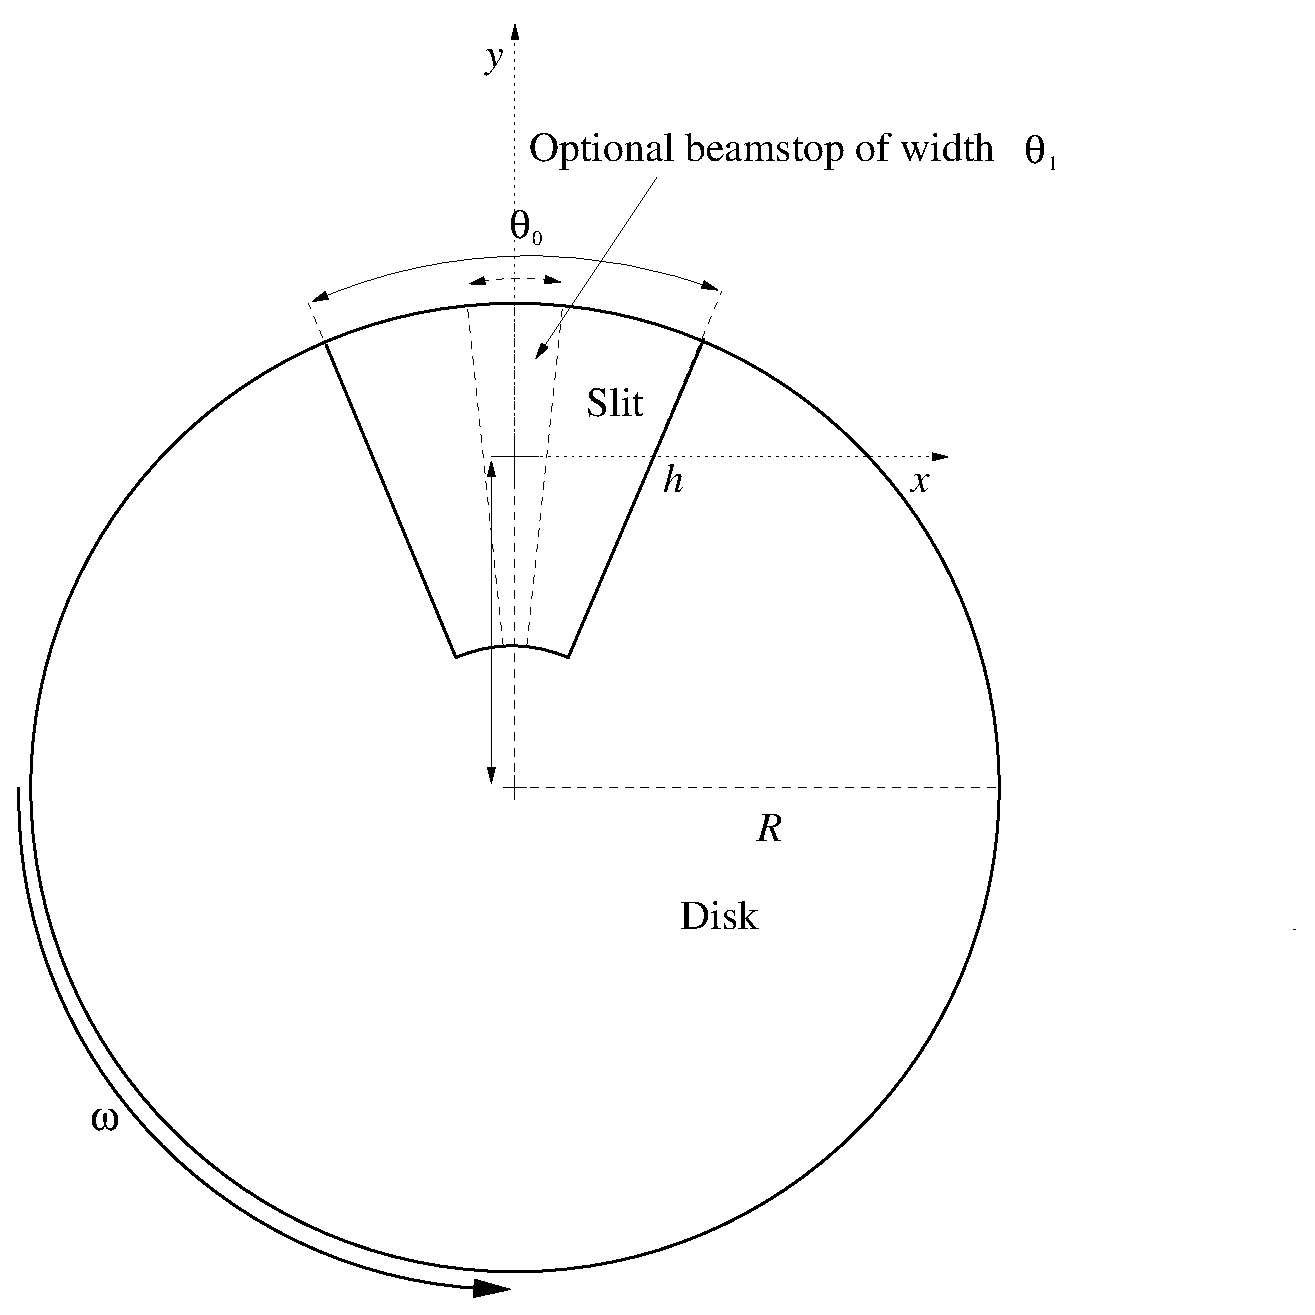
\includegraphics[width=0.8\linewidth]{figures/DiskChopper.eps}
\caption{Sketch of a disc chopper with geometry parameters} 
\label{f:chopper1}
\end{figure}


%Using a rectangular shaped beam with nearly the same
%size as the slit, yields an almost triangular shaped
%transmission curve (see figure~\ref{f:chopper2}).
%
%\begin{figure}[ht]
%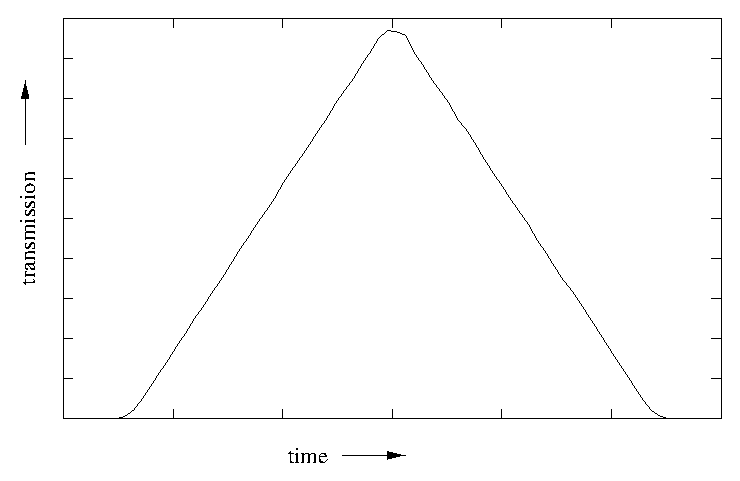
\includegraphics[width=1.0\linewidth]{figures/tracho.eps}
%\caption{example transmission curve for the disc chopper\label{f:chopper2}}
%\end{figure}

When simulating the chopping of a continuous beam,
most of the neutrons could easily be lost.
To improve efficiency, one can set the flag \verb+IsFirst+, which will
allow every neutron ray to pass the {\bf DiskChopper}, but modify the
time, $t$, to a (random) time at which it is possible to pass.
%This can also be used with TOF-instruments, which often
%define the starting time of the neutrons at
%the position of the first chopper.
Of course, there should be only one ``first chopper'' in
any simulation.
To simulate frame overlap from a ``first chopper'', one can specify
the number of frames to study by the parameter $n_{\rm pulse}$.

For more advanced chopper geometries than those mentioned above, it is
possible to set up a \texttt{GROUP} of choppers:

\begin{verbatim}
COMPONENT Chop1 = DiskChopper(omega=2500, R=0.3, h=0.2, theta_0=20, n=1)
AT (0, 0, 1.1) RELATIVE Source
GROUP Choppers

COMPONENT Chop2 = DiskChopper(omega=2500, R=0.3, h=0.2, theta_0=20, n=1,
                              phi_0=40)
AT (0, 0, 1.1) RELATIVE Source
GROUP Choppers
\end{verbatim}

The result of such a {\bf DiskChopper} \texttt{GROUP}ing can be seen in
figure \ref{f:chopper2}

\begin{figure}[ht]
\includegraphics[width=0.4\linewidth]{figures/DiskChopperGroup.ps}
\includegraphics[width=0.4\linewidth]{figures/DiskChopperPSD.eps}
\caption{\texttt{mcdisplay} rendering and monitor output from a DiskChopper \texttt{GROUP}} 
\label{f:chopper2}
\end{figure}